\documentclass[journal]{IEEEtran}

\usepackage{amsmath,amssymb}
\usepackage{graphicx}
\usepackage{booktabs}
\usepackage{multirow}
\usepackage{float}
\usepackage[section]{placeins}
\usepackage{xcolor}
\usepackage[hidelinks,hypertexnames=false]{hyperref}
\hypersetup{
  pdftitle={Collapse-Aware Maintenance of Encrypted Traffic Classifiers under Temporal Drift},
  pdfauthor={Junwei Xiao, Xiaobo Jin, Xiucheng Wu, Zhiquan Liu, Dongjie Liu},
  pdfsubject={Class-aware maintenance of encrypted traffic classifiers under temporal drift}
}
\usepackage{algorithm}
\usepackage{algorithmic}
\usepackage{pgfplots}
\pgfplotsset{compat=1.18}
\setlength{\emergencystretch}{2em}

\graphicspath{{./}}

\newcommand{\ours}{CARE}  % Collapse-Aware REpair
\newcommand{\ie}{\textit{i.e.}}
\newcommand{\eg}{\textit{e.g.}}
\newcommand{\etal}{\textit{et al.}\@}

\begin{document}

\title{Collapse-Aware Maintenance of Encrypted Traffic Classifiers under Temporal Drift}

\author{Junwei Xiao, Xiaobo Jin, Xiucheng Wu, Zhiquan Liu, and Dongjie Liu%
\thanks{Junwei Xiao, Zhiquan Liu, and Dongjie Liu are with the College of Cyber Security, Jinan University, Guangzhou 511443, China (e-mail: xjw20528@stu2024.jnu.edu.cn; zqliu@vip.qq.com; djliu@jnu.edu.cn).}%
\thanks{Xiaobo Jin is with the Department of Intelligent Science, School of Advanced Technology, Xi'an Jiaotong-Liverpool University, Suzhou 215123, China (e-mail: Xiaobo.Jin@xjtlu.edu.cn).}%
\thanks{Xiucheng Wu is with Coremail, Guangzhou 510006, China (e-mail: mwu@coremail.cn).}%
\thanks{Dongjie Liu is the corresponding author.}}

\maketitle

\begin{abstract}
Traffic-based inference supports device management and security monitoring in Internet of Things (IoT) networks, where evolving traffic calls for reliable classifier maintenance. We examine longitudinal encrypted application traffic, where aggregate metrics can conceal severe class-specific failures. We formalize absorber collapse, a class-asymmetric failure in which dominant classes absorb predictions from victim classes and drive their recall toward zero. On CESNET-TLS-Year22, 12 of 178 classes collapse within nine months, while five tested traffic-adapted test-time adaptation methods leave collapse-class F1 below 0.031. We propose Collapse-Aware Repair (CARE), which combines unsupervised class-health monitoring with head-only repair using newly labeled target samples, all-class reference replay, and knowledge distillation. With Batch Active Learning by Diverse Gradient Embeddings (BADGE), CARE raises macro-F1 from 0.629 to 0.700 and collapse-class F1 from 0.028 to 0.332 using 1{,}000 target labels under strict query-excluded evaluation over five repair seeds, while retaining stable-class F1 near the static level (0.894 versus 0.903). A QUIC stress test probes cross-protocol transfer. A separate 11-household IoT device-type holdout shows low-recall-class recovery alongside heterogeneous gains and losses across homes, underscoring the need to review candidate updates at the class level.
\end{abstract}

\begin{IEEEkeywords}
Encrypted traffic classification, IoT traffic analytics, concept drift, class collapse, label-efficient maintenance, active learning.
\end{IEEEkeywords}

% ============================================================

\section{Introduction}
\label{sec:intro}

Traffic-based inference supports device inventory and network monitoring in IoT environments even when payloads are unavailable. Residential studies document temporal and cross-home drift in device-type inference~\cite{pashamokhtari2023dynamic,azizi2025labelshift,azizi2026budget}. A central maintenance question extends across traffic-classification tasks: can aggregate accuracy conceal the failure of individual classes, and can a small number of fresh labels repair them without damaging the others? We investigate this question primarily with longitudinal encrypted application traffic and examine its reach in a separate 11-household IoT device-type setting.

Encrypted-traffic classifiers degrade as applications, protocols, and infrastructure evolve~\cite{soukup2025drift,malekghaini2023drift}. We identify a class-asymmetric pattern, termed \textit{absorber collapse}, in which a dominant predicted class attracts traffic from another class until the latter has near-zero recall. A model can therefore retain acceptable macro-F1 while no longer recognizing a particular class. Such failures matter when class predictions inform network monitoring or policy. High-confidence errors are difficult to correct with entropy-based test-time adaptation (TTA) or pseudo-labeling: both can reinforce the wrong absorber prediction.

We propose \ours{} (Collapse-Aware REpair), an operator-reviewed maintenance workflow. An unlabeled class-health monitor ranks potential failures; after review, Margin or BADGE selects target flows for labeling. A frozen encoder and a fine-tuned classification head use those labels together with all-class reference replay and source-head distillation. The repair is evaluated for both collapsed-class recovery and stable-class preservation. Figure~\ref{fig:care_workflow} places this workflow in a possible IoT traffic-analytics system; the household experiment tests its repair stage, not a deployed gateway.

Our contributions are threefold: (1) a longitudinal characterization of absorber collapse and its empirical signatures; (2) a label-efficient, class-aware repair procedure with explicit preservation of unaffected classes; and (3) strict query-excluded evaluation across time, adapted baselines, a QUIC stress test, and a separate 11-home device-type study that reveals the limits of cross-household transfer. The latter uses a different label space and training protocol; its mixed outcomes are reported as an external stress test rather than as universal IoT efficacy.

% ============================================================


\section{Related Work}
\label{sec:related}

Temporal and cross-home shifts in IoT device traffic motivate model selection, class-prior adaptation, and budget-aware labeling~\cite{pashamokhtari2023dynamic,azizi2025labelshift,azizi2026budget}. Longitudinal encrypted-traffic studies likewise document changing class behavior~\cite{soukup2025drift,malekghaini2023drift,jerabek2025eval}. Our focus is the narrower failure in which an existing class becomes nearly unrecognizable while aggregate performance can remain usable.

Label-free TTA methods such as Tent, EATA, SAR, CoTTA, and NOTE~\cite{wang2021tent,niu2022eata,niu2023sar,wang2022cotta,gong2022note} adapt to distribution shift, but confident absorber errors provide little entropy-based corrective signal. Self-evolving traffic adaptation~\cite{chen2025selfevolving} uses high-confidence pseudo-labels; its collapse-specific recovery was not reported. Domain alignment~\cite{ganin2016dann,long2018cdan} and continual-learning methods~\cite{cerasuolo2024memento,zhu2023iletc,prime2025} address broader adaptation or forgetting, while our fixed-label-space task requires recovery and preservation together.

Active learning allocates scarce labels through uncertainty or diversity~\cite{settles2009active,sener2018coreset,ash2020badge}. Traffic-oriented drift and active-learning studies~\cite{yang2021cade,micfoal2023,netguard2025} address adjacent tasks. \ours{} combines class-level monitoring, target-label acquisition, and reference-based head repair; we compare its components and adapted baselines under stated budgets and protocols.

% ============================================================


\section{Empirical Analysis: Class Collapse Under Drift}
\label{sec:analysis}

\subsection{Problem Formulation}
\label{sec:problem}

Let $f_\phi: \mathcal{X} \to \mathbb{R}^d$ denote a frozen feature encoder and $h_\theta: \mathbb{R}^d \to \mathbb{R}^C$ a classification head, jointly trained on a source period $\mathcal{D}^{\text{src}}$ with $C$ application classes.
At a later target period $t$, the data distribution shifts: $P_t(\mathbf{x}, y) \neq P_{\text{src}}(\mathbf{x}, y)$.
We define a class $c$ as \textit{collapsed} at period $t$ if its recall $R_c^{(t)} = \text{TP}_c / ({\text{TP}_c + \text{FN}_c}) < \tau$, where TP and FN denote true positives and false negatives; we use $\tau{=}0.1$.
A collapsed class $c$ has a \textit{primary absorber} $a(c) = \arg\max_{j \neq c}\, n_{c \to j}$, where $n_{c \to j}$ counts samples with true label $c$ predicted as $j$.
The goal is to update $h_\theta$ using a small label budget $B \ll |\mathcal{D}^{\text{tgt}}|$ and optional reference-period replay, recovering collapsed classes while preserving stable-class performance.


\subsection{Longitudinal Analysis Setup}
\label{sec:setup_analysis}

CESNET-TLS-Year22~\cite{hynek2024cesnet} provides 12 monthly partitions of encrypted application flows. We use the DataZoo \texttt{size=S} split (178 classes), with 1{,}323{,}229 M12 target instances represented by the first 30 packet sizes, directions, and inter-packet times. A three-layer 1D CNN with GroupNorm and a 256-dimensional representation is trained on M3 and evaluated on M4--M12. Source training uses cross-entropy and three auxiliary self-supervised tasks for 30 epochs with AdamW (learning rate $10^{-3}$, batch size 1024). The encoder remains frozen during repair. The separate household study evaluates device-type labels.

\subsection{The Absorber-Collapse Pattern}
\label{sec:absorber}

\begin{figure}[!htbp]
\centering
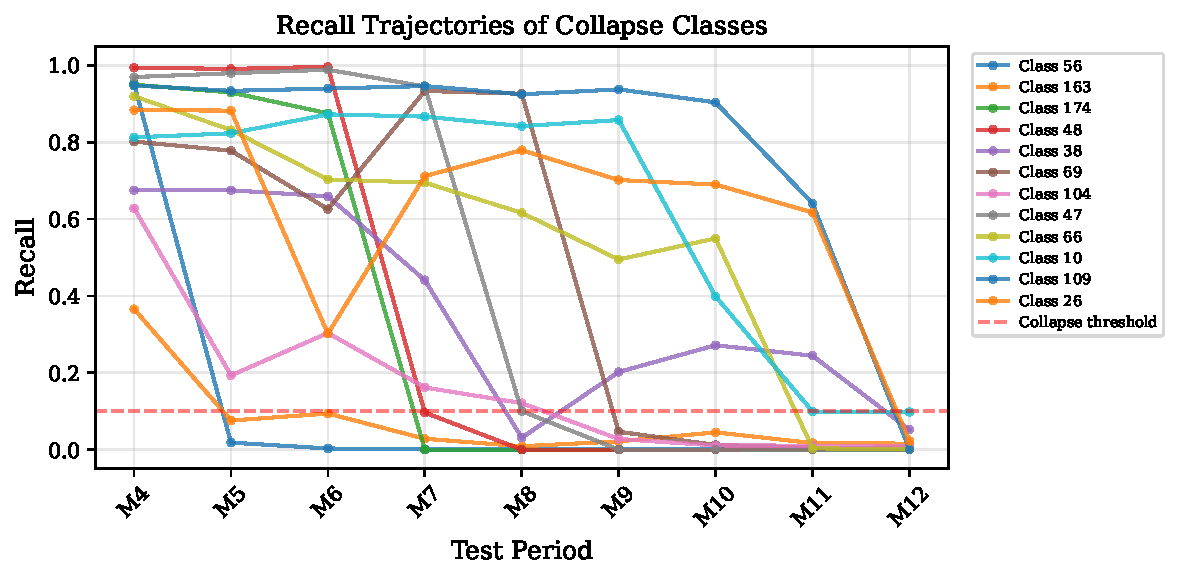
\includegraphics[width=\columnwidth]{fig_collapse_timeline.pdf}
\caption{Recall trajectories of 12 collapse classes on CESNET-TLS-Year22. Classes exhibit both abrupt collapse (\eg{}, class~56 at M5) and gradual decline (\eg{}, class~104 over M4--M12). By M12, all 12 classes fall below the 0.1 recall threshold (dashed line).}
\label{fig:collapse_timeline}
\end{figure}


Figure~\ref{fig:collapse_timeline} shows abrupt failure (class~56: recall 0.952 at M4 to 0.018 at M5) and gradual failure (class~104: 0.629 at M4 to 0.010 at M12). Each collapsed victim has a primary predicted absorber; Table~\ref{tab:absorber_pairs} lists the 12 M12 pairs, whose dominant confusion rates range from 13.9\% to 46.1\%.

\begin{table}[!htbp]
\centering
\caption{Absorber-collapse pairs at M-2022-12. Each collapsed class has a dominant confusion target (absorber). Confusion rate = fraction of victim samples predicted as the absorber.}
\label{tab:absorber_pairs}
\small
\begin{tabular}{@{}cccccc@{}}
\toprule
Victim & Absorber & Confusion & Victim & Pattern & First \\
Class  & Class    & Rate      & Recall & Type    & Collapse \\
\midrule
56  & 96  & 25.2\% & 0.000 & abrupt  & M5 \\
163 & 46  & 41.8\% & 0.015 & gradual & M5 \\
174 & 2   & 29.2\% & 0.000 & abrupt  & M7 \\
48  & 14  & 39.0\% & 0.001 & abrupt  & M7 \\
38  & 45  & 46.1\% & 0.052 & abrupt  & M8 \\
69  & 105 & 37.7\% & 0.005 & abrupt  & M9 \\
104 & 2   & 21.2\% & 0.010 & gradual & M9 \\
47  & 5   & 45.1\% & 0.000 & gradual & M11 \\
66  & 71  & 13.9\% & 0.001 & abrupt  & M11 \\
10  & 156 & 36.5\% & 0.098 & gradual & M11 \\
109 & 71  & 24.9\% & 0.000 & abrupt  & M12 \\
26  & 13  & 21.6\% & 0.022 & abrupt  & M12 \\
\bottomrule
\end{tabular}
\end{table}


\subsection{Two Empirical Signatures of Collapse}
\label{sec:mechanisms}

We compare victim--absorber Fisher discriminant ratios at M4 and M12. Nine pairs show reduced separability (relative decreases of 14--59\%); three show increased separation (30--45\%) despite continued absorption by the frozen head. The latter is consistent with a boundary mismatch. These descriptive signatures suggest that target-label boundary repair and broad class preservation are both relevant, but do not identify causal shift mechanisms.


\subsection{Why General TTA Methods Fail}
\label{sec:tta_eval}

We adapt Tent, EATA, SAR, CoTTA, and NOTE to 1D packet sequences; EATA, CoTTA, and NOTE require simplified traffic-specific components. All five leave M12 collapse F1 below 0.031 in Table~\ref{tab:main_results}, including across five learning rates from $10^{-5}$ to $10^{-3}$. When the model confidently predicts an absorber for a victim, minimizing entropy supplies no signal for the correct victim class. The implementation adaptations limit conclusions about the original methods, but the shared negative result motivates verified target labels.

% ============================================================

\section{Method: Collapse-Aware Repair}
\label{sec:method}


\ours{} combines an unlabeled class-health monitor, active target-label acquisition, and head repair with all-class replay and distillation (Algorithm~\ref{alg:care}). Figure~\ref{fig:care_workflow} places these steps in a proposed operator-reviewed traffic-analytics workflow. The household experiment in Section~\ref{sec:iot_homes} evaluates repair on device types; it does not implement a gateway.

\begin{figure*}[!t]
\centering
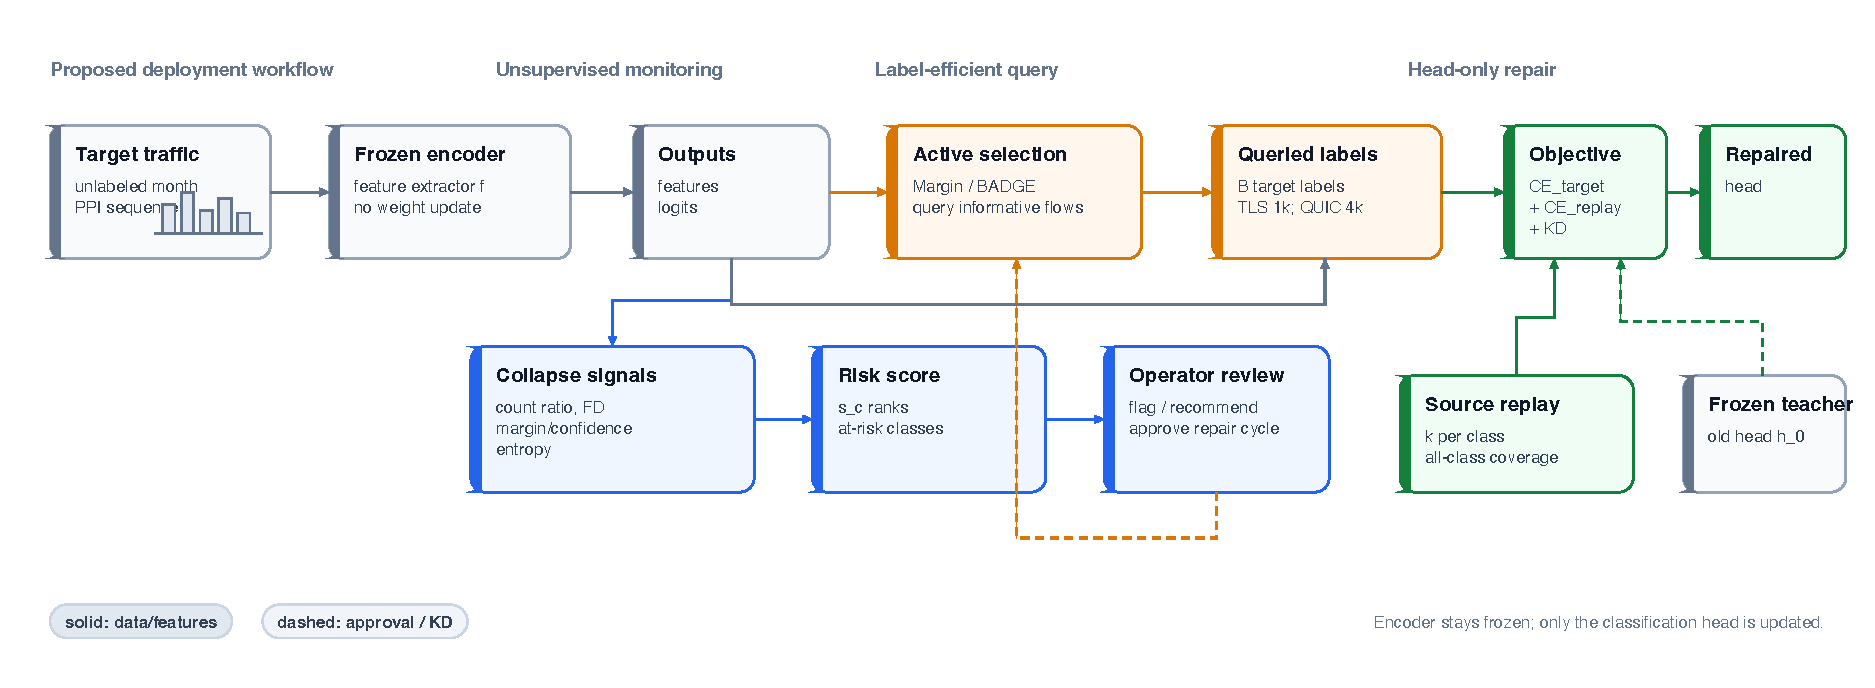
\includegraphics[width=\textwidth]{fig_care_workflow_v4.pdf}
\caption{Proposed operator-reviewed \ours{} workflow. A frozen encoder produces target-period logits and features. Monitoring ranks class-level risk and flags classes for operator review; only an approved repair cycle proceeds to active label selection and offline head-only repair with all-class reference-period replay and knowledge distillation.}
\label{fig:care_workflow}
\end{figure*}


\subsection{Unsupervised Collapse Detection and Monitoring}
\label{sec:unsup_detect}


For each class $c$, the monitor compares reference and target predictions using five unlabeled signals: predicted-class count ratio $r_c=(n_c^{\mathrm{tgt}}/N^{\mathrm{tgt}})/(n_c^{\mathrm{ref}}/N^{\mathrm{ref}})$, Fr\'{e}chet feature distance, mean margin drop, mean confidence drop, and mean entropy rise. The score is
\begin{equation}
 s_c=0.40\max(0,1-r_c)+0.20\tilde d_c+0.15\tilde m_c+0.15\tilde f_c+0.10\tilde e_c,
\end{equation}
where tildes denote median-absolute-deviation-normalized signals. We flag scores above 0.12, retaining at most 20 classes for operator review. Weights and threshold are fixed heuristics; Section~\ref{sec:detection_eval} reports diagnostic performance. The monitor does not select replay classes, which always cover the full label space.

\subsection{Active Sample Selection}
\label{sec:sample_select}


We select $B$ target flows for labeling. Margin ranks globally small top-two logit gaps; BADGE~\cite{ash2020badge} combines uncertainty and gradient-embedding diversity. Our BADGE implementation uses top-three-class gradient embeddings, 50-dimensional principal component analysis, and $B$ k-means++ seeding steps. Both selectors use the same subsequent repair procedure.

\subsection{Head Fine-Tuning with All-Class Reference-Period Replay}
\label{sec:ft_replay}


We precompute frozen features $z=f(x)$ and update only the head $h_\theta$. The training multiset contains $\rho$ copies of each queried target feature and $k=5$ labeled reference features per class (890 total for TLS; default $\rho=2$). Its cross-entropy loss is
\begin{equation}
 \mathcal L_{\mathrm{ft}}=|D_{\mathrm{train}}^z|^{-1}\sum_{(z,y)\in D_{\mathrm{train}}^z}\ell_{\mathrm{CE}}(h_\theta(z),y).
\end{equation}
At $B=1{,}000$, this uses 1{,}000 newly labeled target flows and 2{,}890 training entries after repetition and replay.

\subsection{Knowledge Distillation}
\label{sec:distill}

On replay feature exemplars, we add a KL-divergence loss~\cite{hinton2015distilling} between the updated head $h_\theta$ and original head $h_{\theta_0}$:
\begin{equation}
  \mathcal{L}_{\text{KD}} = \frac{T^2}{|D_{\text{replay}}^z|} \!\sum_{z \in D_{\text{replay}}^z} D_{\text{KL}}\!\!\left(\sigma\!\!\left(\frac{h_{\theta_0}(z)}{T}\right) \!\Big\|\! \sigma\!\!\left(\frac{h_\theta(z)}{T}\right)\!\right)
\end{equation}
where $T$ is the temperature and $\sigma$ is softmax. The $T^2$ factor matches the implementation. Each update independently samples a reference minibatch with replacement for distillation.
Distillation is applied only on replay features because the teacher's reference-period predictions represent its source behavior.
On target samples, the teacher's predictions may already reflect absorber-collapse errors, making them unsuitable as distillation targets.

\subsection{Combined Objective and Algorithm}

The full training loss is:
\begin{equation}
  \mathcal{L} = \mathcal{L}_{\text{ft}} + \lambda_{\text{KD}} \cdot \mathcal{L}_{\text{KD}}
\end{equation}

\begin{algorithm}[t]
\caption{\ours{}: Collapse-Aware Repair}
\label{alg:care}
\begin{algorithmic}[1]
\REQUIRE Source model $f, h_{\theta_0}$; labeled reference features and reference predictions; unlabeled target data $D_{\text{tgt}}$; budget $B$; repeat $\rho$; epochs $E$
\STATE \textbf{Monitor:} Compute per-class risk scores $s_c$ (\S\ref{sec:unsup_detect}) from unlabeled predictions
\STATE \textbf{Alert:} Flag risk for operator review; proceed only after operator approval
\STATE Compute features and logits for $D_{\text{tgt}}$
\STATE Select $B$ samples via margin or BADGE; query labels $\to D_{\text{tgt}}^z$
\STATE Sample $D_{\text{replay}}^z$: $k{=}5$ frozen features from labeled reference-period data for all 178 classes
\STATE Build $D_{\text{train}}^z$ with $\rho$ target copies and one reference copy
\STATE Initialize $h_\theta \leftarrow h_{\theta_0}$
\FOR{epoch $= 1, \ldots, E$}
  \FOR{minibatch in a shuffled pass over $D_{\text{train}}^z$}
    \STATE Independently sample a reference minibatch for KD
    \STATE $\mathcal{L} \leftarrow \mathcal{L}_{\text{ft}} + \lambda_{\text{KD}} \cdot \mathcal{L}_{\text{KD}}$
    \STATE Update $\theta$ via AdamW on $\mathcal{L}$
  \ENDFOR
\ENDFOR
\RETURN Updated classifier $h_\theta$
\end{algorithmic}
\end{algorithm}


% ============================================================
\section{Experiments}
\label{sec:experiments}

This section evaluates \ours{} through overall repair performance and baseline comparisons, internal mechanisms, cross-setting stress tests, and diagnostic detection quality. We first describe the primary datasets, evaluation protocols, metrics, and implementation settings; the distinct IoT household protocol is specified with its results.

\subsection{Experimental Setup}
\label{sec:exp_setup}


\textbf{Datasets and protocol.} CESNET-TLS-Year22~\cite{hynek2024cesnet} is the primary 178-class benchmark (M3 source; M7, M9, M11, M12 targets). CESNET-QUICEXT-25 XS~\cite{cesnetquicext25,mucke2025waiting} provides a 44-class cross-protocol test (M-2024-6 to M-2025-5). The TLS dataset also contains a documented flow-exporter change near week 10~\cite{hynek2024cesnet}; our evaluation measures the combined temporal shift. In the main \textit{strict} protocol, queried target flows are excluded from evaluation. A separate seed-matched protocol holds out 20\% before adaptation. Static/TTA rows use one fixed source checkpoint; active rows average five repair seeds. Other seed counts are stated where used.

\textbf{Comparisons and metrics.} We test five unlabeled TTA variants, a Chen-inspired pseudo-label baseline~\cite{chen2025selfevolving}, entropy/coreset/random selectors, and adapted continual-learning methods. Labeled comparisons use the same $B=1{,}000$ budget unless stated otherwise. We report macro-F1; F1 of the 12 M12 classes with static recall $<0.1$ (Col.); F1 of a fixed 20-class M4--M12 stable diagnostic set (Stb.); and the number of those 12 classes still below 0.1 recall (\#Col.). Stable classes are selected retrospectively by the smallest absolute F1 change among classes with $\geq100$ M12 instances and M4 support; this is a preservation endpoint, not a prospective detection set. Per-class recovery is full at recall $\geq0.30$, partial at $0.05$--$0.30$, and failed below 0.05.

\textbf{Source training and exclusion.} The 1D CNN uses three convolutional layers with GroupNorm and a 256-dimensional hidden representation. It is trained for 30 epochs with AdamW; the selected source checkpoint is fixed across primary repair seeds. Query IDs are removed before strict target evaluation, and the five seeds repeat repair rather than source-model training. The 20-class stable endpoint is reported separately from the 12-class collapse endpoint so that recovery does not hide collateral damage.

\textbf{CARE settings.} Unless specified, $B=1{,}000$, five M4 reference features per class, target repeat $\rho=2$, distillation weight $\lambda_{\mathrm{KD}}=0.5$, temperature $T=2$, and 30 head-update epochs with learning rate $10^{-3}$.

\subsection{Overall Performance}
\label{sec:main_results}


\subsubsection{Primary Results under Strict Query-Excluded Evaluation}
\label{sec:primary_results}
Table~\ref{tab:main_results} compares methods nine months after TLS source training.

\begin{table}[!htbp]
\centering
\caption{Main results on CESNET-TLS-Year22 at M-2022-12. Static/TTA rows are single-checkpoint evaluations without labels. Active rows use $B{=}1{,}000$ labels, M4 all-class replay ($k{=}5$, 890 features), KD ($\lambda{=}0.5$), strict query exclusion, and five seeds.}
\label{tab:main_results}
\scriptsize
\setlength{\tabcolsep}{3pt}
\begin{tabular}{@{}l cccc@{}}
\toprule
Method & Macro & Col.\ F1 & Stb.\ F1 & \#Col \\
\midrule
\multicolumn{5}{l}{\textit{No labeled target data:}} \\
Static          & 0.629 & 0.028 & 0.903 & 12 \\
Tent            & 0.631 & 0.026 & 0.903 & 12 \\
EATA            & 0.629 & 0.028 & 0.903 & 12 \\
SAR             & 0.629 & 0.026 & 0.901 & 11 \\
CoTTA           & 0.630 & 0.027 & 0.903 & 12 \\
NOTE            & 0.630 & 0.027 & 0.902 & 12 \\
\midrule
\multicolumn{5}{l}{\textit{Active ($B$=1000, all-class replay+KD, 5 seeds):}} \\
Entropy         & 0.628$\pm$0.004 & 0.078$\pm$0.015 & 0.887$\pm$0.004 & 10.2 \\
Coreset         & 0.633$\pm$0.005 & 0.116$\pm$0.042 & 0.886$\pm$0.007 & 8.8 \\
Random          & 0.668$\pm$0.004 & 0.188$\pm$0.024 & 0.892$\pm$0.006 & 8.2 \\
\ours{}-Margin  & 0.686$\pm$0.001 & 0.256$\pm$0.009 & 0.892$\pm$0.003 & 5.8 \\
\textbf{\ours{}-BADGE} & \textbf{0.700$\pm$0.003} & \textbf{0.332$\pm$0.040} & \textbf{0.894$\pm$0.004} & \textbf{4.0} \\
\bottomrule
\end{tabular}
\end{table}


CARE-BADGE reaches $0.700\pm0.003$ macro-F1 and $0.332\pm0.040$ collapse F1, compared with static values 0.629 and 0.028; its stable-class F1 is 0.894 versus 0.903 static. Margin reaches 0.686 macro-F1 and 0.256 collapse F1 at lower selection cost. The five TTA methods leave collapse F1 below 0.031. Paired $t$-tests favor Margin over Random and BADGE over Margin, but with five seeds exact two-sided Wilcoxon tests cannot resolve either difference at 0.05.

\subsubsection{Matched Holdout and Self-Evolving Baseline}
\label{sec:matched_holdout}
In a separate five-seed experiment, 20\% of the M12 pool is held out before adaptation. A Chen-inspired full-model pseudo-label baseline~\cite{chen2025selfevolving} uses no human target labels; a $p\geq0.997$ confidence setting reaches 0.505 macro-F1 and 0.001 collapse F1, while the post-hoc best-macro $p\geq0.90$ sensitivity setting reaches 0.614 and 0.014. CARE-BADGE, with 1{,}000 verified labels and head-only repair, reaches $0.701\pm0.007$ and $0.310\pm0.047$ on identical seed-wise holdouts. The supervision and update budgets differ, so this is a practical comparison rather than an isolated component effect. Table~\ref{tab:matched_holdout} reports the full matched comparison and program wall time; S1 supplies the archived records.

\begin{table*}[!htbp]
\centering
\caption{Seed-matched 20\% holdout comparison at M12 (mean $\pm$ sample standard deviation over 5 seeds). Human labels count unique queried target labels; pseudo-labels are the mean high-confidence target samples used for our Chen-style full-model fine-tuning. Program wall time is measured on one NVIDIA L20 under each method's final configuration; dashes denote configurations not included in the timing run.}
\label{tab:matched_holdout}
\scriptsize
\resizebox{\textwidth}{!}{%
\begin{tabular}{@{}l rr ccccc@{}}
\toprule
Method & Human & Pseudo & Macro F1 & Collapse F1 & Stable F1 & \#Col. & Wall (s) \\
\midrule
Static & 0 & 0 & $0.6308{\pm}0.0020$ & $0.0313{\pm}0.0055$ & $0.9019{\pm}0.0015$ & 11.8 & -- \\
Chen-style ($p{\geq}0.997$) & 0 & 298.8K & $0.5050{\pm}0.0097$ & $0.0008{\pm}0.0018$ & $0.8063{\pm}0.0208$ & 12.0 & $80.0{\pm}1.0$ \\
Chen-style ($p{\geq}0.90$, sensitivity) & 0 & 628.7K & $0.6140{\pm}0.0058$ & $0.0136{\pm}0.0035$ & $0.8887{\pm}0.0080$ & 12.0 & $136.4{\pm}0.5$ \\
\midrule
\ours{}-Entropy & 1{,}000 & 0 & $0.6316{\pm}0.0025$ & $0.0797{\pm}0.0097$ & $0.8863{\pm}0.0039$ & 10.0 & -- \\
\ours{}-Random & 1{,}000 & 0 & $0.6722{\pm}0.0021$ & $0.2246{\pm}0.0370$ & $0.8934{\pm}0.0039$ & 7.0 & -- \\
\ours{}-Margin & 1{,}000 & 0 & $0.6885{\pm}0.0022$ & $0.2835{\pm}0.0185$ & $0.8932{\pm}0.0047$ & \textbf{4.6} & $48.5{\pm}0.8$ \\
\ours{}-BADGE & 1{,}000 & 0 & $\mathbf{0.7008{\pm}0.0068}$ & $\mathbf{0.3099{\pm}0.0473}$ & $\mathbf{0.9004{\pm}0.0042}$ & 4.8 & $166.6{\pm}8.2$ \\
\bottomrule
\end{tabular}}
\end{table*}

\subsubsection{Comparison with Continual Learning Baselines}
\label{sec:cl_baselines}


We adapt MEMENTO~\cite{cerasuolo2024memento} (full-model update with replay and KD), ILETC~\cite{zhu2023iletc} (generated or real replay without KD), CADE-score~\cite{yang2021cade} (drift-score query selection), and an expanded head inspired by PRIME~\cite{prime2025}. All use the strict protocol, five seeds, and 1{,}000 labels; other than CADE-score and CARE-BADGE, they share Margin queries. The adaptations are task-specific implementations, not exact reproductions.

\begin{table}[!htbp]
\centering
\caption{Continual-learning and drift-adaptation baselines at M-2022-12 ($B{=}1{,}000$, strict eval, 5 seeds). CADE-score and CARE-BADGE use their named selectors; other labeled rows use Margin. CARE rows are reproduced from Table~\ref{tab:main_results}.}
\label{tab:cl_baselines}
\scriptsize
\setlength{\tabcolsep}{3pt}
\begin{tabular}{@{}l cccc@{}}
\toprule
Method & Macro & Col.\ F1 & Stb.\ F1 & \#Col \\
\midrule
Static & 0.629 & 0.028 & \textbf{0.903} & 12.0 \\
\midrule
\multicolumn{5}{l}{\textit{CL / drift baselines (same label budget):}} \\
CADE-score~\cite{yang2021cade}     & 0.637$\pm$0.004 & 0.118$\pm$0.015 & 0.889$\pm$0.003 & 9.0 \\
ILETC-GAN~\cite{zhu2023iletc}     & 0.650$\pm$0.004 & 0.219$\pm$0.010 & 0.851$\pm$0.009 & 5.4 \\
ILETC-real                         & 0.659$\pm$0.003 & 0.236$\pm$0.010 & 0.854$\pm$0.016 & 4.8 \\
Expanded head                      & 0.673$\pm$0.003 & 0.307$\pm$0.005 & 0.871$\pm$0.008 & 4.8 \\
MEMENTO~\cite{cerasuolo2024memento}& 0.678$\pm$0.002 & 0.255$\pm$0.005 & 0.892$\pm$0.004 & 6.0 \\
\midrule
\ours{}-Margin & 0.686$\pm$0.001 & 0.256$\pm$0.009 & 0.892$\pm$0.003 & 5.8 \\
\textbf{\ours{}-BADGE} & \textbf{0.700$\pm$0.003} & \textbf{0.332$\pm$0.040} & 0.894$\pm$0.004 & \textbf{4.0} \\
\bottomrule
\end{tabular}
\end{table}


Table~\ref{tab:cl_baselines} shows that CARE-BADGE has the highest mean macro-F1 and collapse F1 among these rows. MEMENTO reaches 0.678/0.255; the expanded head reaches 0.673/0.307 but has lower stable F1 (0.871). ILETC variants retain less stable-class performance (0.851--0.854). These contrasts support the bounded head-update and preservation design in this setting, without isolating every architectural or loss difference.

\subsubsection{Multi-Period Generalization}
\label{sec:multi_period}

Table~\ref{tab:multiperiod} evaluates Margin-based repair at four drift periods.

\begin{table}[!htbp]
\centering
\caption{Multi-period results (Margin, $B$=1000, all-class replay $k{=}5$, 3 seeds). The fixed collapse set is the 12 classes identified by the M12 static model.}
\label{tab:multiperiod}
\scriptsize
\setlength{\tabcolsep}{3pt}
\begin{tabular}{@{}l cc cc c@{}}
\toprule
& \multicolumn{2}{c}{Static} & \multicolumn{2}{c}{\ours{}} & \\
\cmidrule(lr){2-3} \cmidrule(lr){4-5}
Period & Macro & Col. & Macro & Col. & $\Delta$ Macro \\
\midrule
M7 (light)   & 0.740 & 0.503 & 0.776$\pm$0.003 & 0.633$\pm$0.028 & +0.036 \\
M9 (medium)  & 0.691 & 0.280 & 0.739$\pm$0.003 & 0.392$\pm$0.005 & +0.048 \\
M11 (heavy)  & 0.649 & 0.145 & 0.708$\pm$0.002 & 0.408$\pm$0.016 & +0.060 \\
M12 (severe) & 0.629 & 0.028 & 0.686$\pm$0.002 & 0.255$\pm$0.012 & +0.057 \\
\bottomrule
\end{tabular}
\end{table}


Macro-F1 and fixed-group collapse F1 improve at all four periods. The M12 macro-F1 gain is 0.057; earlier intervention at M7 yields 0.633 collapse F1. These are independent monthly repairs, not a sequential deployment.

\subsection{Internal Mechanism Analysis}
\label{sec:mechanism_analysis}


\subsubsection{Component-Variant Study}
\label{sec:ablation}
Table~\ref{tab:ablation} compares seven evaluated bundles under Margin queries and five seeds. It is not factorial: repeat factors and replay coverage vary, so its rows do not isolate individual loss effects.

\begin{table*}[!htbp]
\centering
\caption{Component variants at M12 (Margin, strict evaluation, 5 seeds). Targeted-150 contains stable+absorber features; All-890 contains five features per class. FT, Rpl, KD, and Rep. denote fine-tuning, replay, knowledge distillation, and target repeat.}
\label{tab:ablation}
\scriptsize
\setlength{\tabcolsep}{2pt}
\resizebox{\textwidth}{!}{%
\begin{tabular}{@{}l c l c c ccc c@{}}
\toprule
Config. & Target $B$ & Replay & KD & Rep. & Macro & Col.\ F1 & Stb.\ F1 & \#Col \\
\midrule
Static & 0 & None & -- & -- & 0.629 & 0.028 & \textbf{0.903} & 12 \\
\midrule
Replay only & 0 & All-890 & -- & -- & 0.563$\pm$0.007 & 0.044$\pm$0.019 & 0.816$\pm$0.026 & 10.2 \\
Rpl+KD & 0 & All-890 & \checkmark & -- & 0.618$\pm$0.005 & 0.039$\pm$0.016 & 0.888$\pm$0.009 & 10.8 \\
\midrule
FT only & 1000 & None & -- & 1 & 0.638$\pm$0.000 & 0.134$\pm$0.001 & 0.839$\pm$0.001 & 7.0 \\
FT+KD & 1000 & Targeted-150 & \checkmark & 1 & 0.670$\pm$0.000 & 0.152$\pm$0.007 & 0.887$\pm$0.004 & 7.8 \\
FT+Rpl & 1000 & All-890 & -- & 2 & 0.659$\pm$0.003 & 0.236$\pm$0.010 & 0.854$\pm$0.016 & 4.8 \\
\textbf{Full \ours{}} & 1000 & All-890 & \checkmark & 2 & \textbf{0.686$\pm$0.001} & \textbf{0.256$\pm$0.009} & 0.892$\pm$0.003 & 5.8 \\
\bottomrule
\end{tabular}}
\end{table*}





Without target labels, replay variants leave collapse F1 below 0.05. Target-only fine-tuning reaches 0.134 but reduces stable F1 to 0.839; the full Margin-based configuration reaches 0.256 collapse F1 and 0.892 stable F1. Thus target supervision is associated with recovery and reference-based training with preservation across the tested bundles. Separate matched-update reconstruction controls (S2) qualify the incremental value of reference cross-entropy. Full-model fine-tuning under the same label budget gives 0.678 macro-F1 and 0.256 collapse F1 versus 0.686 and 0.256 for head-only repair.

\subsubsection{Selection Strategy Comparison}
\label{sec:al_baselines}





BADGE attains higher mean collapse F1 than Margin (0.332 versus 0.256) at about 3.4 times the program wall time (167 versus 49 s on one L20). With a fixed selector, Margin yields 4 fully recovered, 3 partially recovered, and 5 failed classes; BADGE yields 5, 5, and 2, respectively. Table~\ref{tab:per_class_recovery} shows that many recovered classes receive very few directly labeled examples, consistent with broader boundary updates rather than a positive example for every victim.

\begin{table*}[!htbp]
\centering
\caption{Per-class recovery at M-2022-12 ($B{=}1{,}000$, all-class replay $k{=}5$, strict eval, 5 seeds; mean $\pm$ sample standard deviation). Selected = mean target labels allocated to that class.}
\label{tab:per_class_recovery}
\scriptsize
\setlength{\tabcolsep}{2pt}
\resizebox{\textwidth}{!}{%
\begin{tabular}{@{}r r r cc cc cc rr@{}}
\toprule
& & & \multicolumn{2}{c}{Static} & \multicolumn{2}{c}{\ours{}-Margin} & \multicolumn{2}{c}{\ours{}-BADGE} & \multicolumn{2}{c}{Selected} \\
\cmidrule(lr){4-5} \cmidrule(lr){6-7} \cmidrule(lr){8-9} \cmidrule(lr){10-11}
Class & Abs. & $n$ & Recall & F1 & Recall & F1 & Recall & F1 & Marg & BADGE \\
\midrule
56  & 96  & 12137 & 0.000 & 0.001 & 0.722$\pm$0.033 & 0.784$\pm$0.008 & \textbf{0.793$\pm$0.017} & \textbf{0.829$\pm$0.021} & 12.0 & 13.6 \\
163 & 46  &  1741 & 0.016 & 0.026 & 0.143$\pm$0.031 & 0.168$\pm$0.024 & \textbf{0.226$\pm$0.140} & \textbf{0.235$\pm$0.123} &  3.0 &  4.8 \\
174 &  2  &  1507 & 0.000 & 0.000 & \textbf{0.195$\pm$0.005} & \textbf{0.262$\pm$0.012} & 0.029$\pm$0.040 & 0.044$\pm$0.060 &  4.0 &  1.6 \\
48  & 14  &  3361 & 0.001 & 0.002 & 0.437$\pm$0.009 & 0.568$\pm$0.007 & \textbf{0.722$\pm$0.234} & \textbf{0.767$\pm$0.146} &  4.0 &  4.8 \\
38  & 45  &   193 & 0.052 & 0.090 & \textbf{0.656$\pm$0.095} & \textbf{0.410$\pm$0.057} & 0.242$\pm$0.277 & 0.210$\pm$0.210 &  3.0 &  1.2 \\
69  & 105 &  1866 & 0.005 & 0.008 & 0.031$\pm$0.017 & 0.042$\pm$0.021 & \textbf{0.157$\pm$0.203} & \textbf{0.177$\pm$0.219} &  3.0 &  2.4 \\
104 &  2  &  1744 & 0.010 & 0.016 & \textbf{0.703$\pm$0.044} & \textbf{0.664$\pm$0.031} & 0.604$\pm$0.154 & 0.594$\pm$0.073 &  8.0 &  3.6 \\
47  &  5  &   618 & 0.000 & 0.000 & 0.002$\pm$0.002 & 0.004$\pm$0.003 & \textbf{0.404$\pm$0.201} & \textbf{0.462$\pm$0.168} &  0.0 &  2.2 \\
66  & 71  &  1955 & 0.001 & 0.002 & 0.001$\pm$0.000 & 0.002$\pm$0.001 & \textbf{0.133$\pm$0.118} & \textbf{0.144$\pm$0.121} &  1.0 &  4.2 \\
10  & 156 &  1004 & 0.098 & 0.162 & 0.074$\pm$0.030 & 0.121$\pm$0.044 & \textbf{0.389$\pm$0.215} & \textbf{0.441$\pm$0.193} &  0.0 &  1.8 \\
109 & 71  &   393 & 0.000 & 0.000 & 0.000$\pm$0.000 & 0.000$\pm$0.000 & 0.000$\pm$0.000 & 0.000$\pm$0.000 &  0.0 &  1.6 \\
26  & 13  &   807 & 0.022 & 0.025 & 0.035$\pm$0.012 & 0.046$\pm$0.011 & \textbf{0.125$\pm$0.140} & \textbf{0.087$\pm$0.069} &  1.0 &  2.6 \\
\midrule
\multicolumn{3}{@{}l}{Macro (12 classes)} & 0.017 & 0.028 & 0.250 & 0.256 & \textbf{0.319} & \textbf{0.332} & & \\
\bottomrule
\end{tabular}%
}
\end{table*}


At $B=2{,}000$ Margin-selected target labels, collapse F1 rises to $0.437\pm0.004$ and the number of collapsed classes falls from 12 to 2; at $B=8{,}000$, collapse F1 reaches $0.609\pm0.007$ while stable-class F1 remains at least 0.887. The budget curve is provided in S1. All main labeled-method comparisons use $B=1{,}000$.

\subsubsection{Replay Strategy Comparison}
\label{sec:replay_ablation}
All-class replay with five features per class yields 0.686 macro-F1. At a matched feature count, targeted replay (about 900 features) yields 0.678; all-class replay with one feature per class (178 total) yields 0.680. These comparisons favor breadth of class coverage over concentrating replay on selected classes. The detector therefore ranks classes for review, not for replay selection. A smaller targeted prototype-replay study retained 98.7\% of exemplar-replay macro-F1 while reducing storage from about 150 to 60 KiB.

\subsection{Generalization and Robustness}
\label{sec:generalization_robustness}


\subsubsection{Architecture Robustness}
\label{sec:robustness}
\label{sec:bn_verify}
\label{sec:transformer}
Replacing GroupNorm with BatchNorm does not remove the collapse problem: BN-Adapt~\cite{schneider2020bn} leaves collapse F1 at 0.032. A targeted-replay CARE-Margin variant raises BN macro/collapse F1 from 0.613/0.030 to 0.665/0.314. A four-layer Transformer~\cite{vaswani2017attention} with the same targeted protocol reaches 0.767/0.401. These architecture controls use a different replay variant from the default CNN experiment.

\subsubsection{Cross-Protocol Generalization}
\label{sec:cross_protocol}

QUICEXT-25 stress test.
\label{sec:quicext25}

CESNET-QUICEXT-25 XS~\cite{cesnetquicext25,mucke2025waiting} provides 44 classes with M-2024-6 source and M-2025-5 target partitions. Three classes (17, 23, 25) newly fall below 0.1 recall; class 21 is excluded because it already fails in the reference period. Table~\ref{tab:quicext25} reports strict query-excluded results across label budgets.

\begin{table}[!htbp]
\centering
\caption{Cross-protocol generalization on CESNET-QUICEXT-25 XS (M-2024-6 $\to$ M-2025-5, 44 classes, 5 seeds). $B$ is the number of queried target labels; strict evaluation excludes them.}
\label{tab:quicext25}
\scriptsize
\setlength{\tabcolsep}{3pt}
\begin{tabular}{@{}l c c c c@{}}
\toprule
Method & $B$ & Macro-F1 & Collapse F1 & \#Col. \\
\midrule
Static & 0 & 0.502 & 0.049 & 3.0 \\
\ours{}-Margin & 1000 & $0.564{\pm}0.003$ & $0.114{\pm}0.002$ & $2.0{\pm}0.0$ \\
\ours{}-BADGE & 1000 & $0.563{\pm}0.006$ & $0.091{\pm}0.017$ & $2.8{\pm}0.45$ \\
\ours{}-Margin & 2000 & $0.577{\pm}0.003$ & $0.126{\pm}0.014$ & $2.0{\pm}0.0$ \\
\ours{}-BADGE & 2000 & $0.578{\pm}0.006$ & $0.144{\pm}0.031$ & $2.2{\pm}0.84$ \\
\ours{}-Margin & 4000 & $0.578{\pm}0.002$ & $0.132{\pm}0.021$ & $1.8{\pm}0.45$ \\
\ours{}-BADGE & 4000 & $\mathbf{0.586{\pm}0.007}$ & $\mathbf{0.191{\pm}0.030}$ & $\mathbf{1.2{\pm}0.45}$ \\
\bottomrule
\end{tabular}
\end{table}


With 1{,}000 labels, CARE-Margin raises macro/collapse F1 from 0.502/0.049 to 0.564/0.114. BADGE at 4{,}000 labels reaches 0.586/0.191. The higher QUIC label requirement motivates protocol-specific budget choice.

\subsubsection{Training-Seed and Checkpoint Robustness}
\label{sec:checkpoint_robustness}

A targeted-replay retraining audit ($3{\times}3{=}9$ runs) yields static macro-F1 of $0.620{\pm}0.001$ and CARE macro-F1 of $0.667{\pm}0.007$ across training seeds.
Our primary checkpoint (static $0.629$, best epoch 27/30, validation F1 $0.892$) is about 0.009 above the audit mean, larger than the audit standard deviation and therefore evidence of checkpoint/run sensitivity. The targeted-replay CARE variant improves over its corresponding static model in all audited training seeds, although the gain magnitude varies.

\subsubsection{Exploratory IoT Device-Type Stress Test}
\label{sec:iot_homes}


We evaluate a public residential IoT flow archive~\cite{pashamokhtari2023dynamic} as a closed-set, mixed-protocol device-type task. The official MAC inventory provides 24 type labels; MAC/IP addresses, ports, timestamps, and labels are excluded from model inputs, which comprise 22 flow statistics and six protocol indicators. Eleven homes contain all 24 source types. Each home uses chronological source, query, development, and final windows split at approximately 50\%, 70\%, and 85\% of observed days, with a separate 28-input tabular MLP. For each home and five overlapping repair seeds, 1{,}000 uniformly sampled query labels and five reference features per class train the ported CARE head. This port differs from the CNN/BADGE main study and evaluates repair without monitoring.

Source training uses a class-capped reservoir (up to 5{,}000 flows per type); the query pool is a uniform reservoir from the subsequent chronological window. The model uses flow statistics and protocol indicators rather than device identifiers, so the IoT experiment tests traffic-based type recognition rather than memorization of MAC addresses. The five repair seeds share each home's source model and are repeated measurements, not additional homes.

Development analyses informed a fixed final comparison of static, target-only, CARE, and standard 0.5 source--target head interpolation (BCWI). Refit predictions were checked against frozen development outputs; final-window predictions and scoring rules were frozen before final labels were decoded. Table~\ref{tab:iot_homes} reports the final per-home results; homes are independent units.

\begin{table*}[!t]
\centering
\caption{IoT device-type final-window holdout on 11 homes. Each home uses a separate source MLP and 1{,}000 uniform paid labels per repair seed; CARE and the fixed source--target head-interpolation control (BCWI 0.50) average five overlapping seeds. Macro-F1 averages device types present in that home's final window. Deltas are percentage points versus the static model, computed before rounding. Homes, rather than seeds, are independent units.}
\label{tab:iot_homes}
\small
\setlength{\tabcolsep}{7pt}
\begin{tabular}{@{}lrrrrr@{}}
\toprule
Home & Static F1 & \ours{} F1 & $\Delta_{\mathrm{CARE}}$ (pp) & BCWI F1 & $\Delta_{\mathrm{BCWI}}$ (pp) \\
\midrule
01 & 0.5895 & 0.6100 & $+2.047$ & 0.6106 & $+2.106$ \\
02 & 0.4623 & 0.4606 & $-0.172$ & 0.4915 & $+2.916$ \\
03 & 0.5201 & 0.5171 & $-0.306$ & 0.5421 & $+2.198$ \\
04 & 0.4327 & 0.4444 & $+1.163$ & 0.4539 & $+2.115$ \\
05 & 0.4498 & 0.4332 & $-1.661$ & 0.4636 & $+1.386$ \\
06 & 0.5470 & 0.4829 & $-6.410$ & 0.5109 & $-3.615$ \\
07 & 0.5536 & 0.5009 & $-5.272$ & 0.4603 & $-9.331$ \\
08 & 0.4930 & 0.5214 & $+2.838$ & 0.5429 & $+4.987$ \\
09 & 0.5564 & 0.5687 & $+1.234$ & 0.6095 & $+5.310$ \\
11 & 0.5553 & 0.5593 & $+0.399$ & 0.5511 & $-0.420$ \\
12 & 0.5609 & 0.5379 & $-2.293$ & 0.5780 & $+1.716$ \\
\midrule
Equal-home mean & 0.52006 & 0.51239 & $-0.767$ & 0.52858 & $+0.852$ \\
\bottomrule
\end{tabular}
\end{table*}


On development windows, CARE improves equal-home macro-F1 from 0.54279 to 0.54424 (6/11 homes). Among 17 low-recall home--type pairs with at least 50 rows, all improve in mean F1 and 11 reach recall at least 0.1; 12 of the 17 receive fewer than five paid positives on average. Among 75 initially high-recall pairs, seven lose more than five F1 points. These outcomes motivated explicit final-window class-level endpoints, without changing CARE training.

On final windows, low-recall-class F1 rises from 0.03988 (static) to 0.13887 (CARE), while equal-home macro-F1 changes from 0.52006 to 0.51239 ($-0.767$ percentage points; five homes improve). The descriptive home-bootstrap interval for the mean difference is $[-2.474,0.756]$ points. CARE's conditional negative-flip rate is 0.05908; it restores recall to at least 0.1 for an average 0.78 of 1.64 low-recall types per home, while 0.42 of 5.55 stable types per home lose more than five F1 points. Target-only and BCWI reach mean macro-F1 of 0.48581 and 0.52858, respectively. No pair meets the stricter development-to-final incident-collapse definition. Preselected home-level shift indicators show no clear association with CARE benefit. This stress test demonstrates device-type recovery alongside whole-model variation and harm in some homes.

\subsection{Diagnostic Detector Evaluation}
\label{sec:detection_eval}


At M12, the five-signal score detects 10 of 12 collapsed classes at precision 0.50 and recall 0.833; count drop plus Fr\'{e}chet distance alone gives 0.45/0.75. Table~\ref{tab:trigger} shows the monitor across drift periods.

\begin{table}[!htbp]
\centering
\caption{Detection across drift levels ($k{=}20$, recall${<}0.1$, support${\geq}50$). GT denotes ground truth; recall is $\geq$0.80 throughout.}
\label{tab:trigger}
\small
\begin{tabular}{@{}l cccc@{}}
\toprule
Period & GT & Precision & Recall & F1 \\
\midrule
M7 (light)   & 5  & 0.200 & 0.800 & 0.320 \\
M9 (medium)  & 8  & 0.350 & 0.875 & 0.500 \\
M11 (heavy)  & 10 & 0.450 & 0.900 & 0.600 \\
M12 (severe) & 12 & 0.500 & 0.833 & 0.625 \\
\bottomrule
\end{tabular}
\end{table}


Detection recall stays at least 0.80 across periods, while precision rises from 0.20 at M7 to 0.50 at M12. Equal and historically calibrated weight variants give M12 detection F1 between 0.563 and 0.625. These are retrospective diagnostic operating points, not an automatic update gate.

% ============================================================


\section{Discussion}
\label{sec:discussion}

\subsection{Class-Level Maintenance}
\label{sec:discussion_efficacy}
The TLS experiments show that verified target labels can recover classes missed by confidence-based adaptation, while reference replay and distillation limit damage to stable classes. CARE-BADGE offers the strongest mean recovery in the primary comparison; Margin has lower selection cost. The QUIC stress test shows the same direction with a larger budget. The IoT holdout exposes the harder acceptance problem: improved recognition of some device types can coexist with losses in other types and homes. A candidate head should therefore be assessed with per-class recovery and harm measures before activation.

\subsection{Operational Scope and Limitations}
\label{sec:discussion_deployment}
\label{sec:discussion_iot}
\label{sec:discussion_limitations}
Figure~\ref{fig:care_workflow} depicts an operator-reviewed cycle: monitor unlabeled traffic, inspect class-risk alerts, acquire limited labels, repair offline, and validate a candidate head while the deployed model continues serving. The evaluated TLS cycle uses 1{,}000 target labels and 890 stored reference features; human review and deployment costs were not measured. The detector prioritizes recall and incurs false alerts, so it is a screening tool. Head-only repair also depends on a usable frozen representation and cannot add unseen classes.

The monitored class-health score is a proposal for human review. Its M12 precision of 0.50 means that even a sensitive alert cannot by itself justify deployment. At a candidate update, the operator can compare per-class confusion and negative flips against the existing model; the IoT holdout shows why this check matters even when a low-recall category recovers. A live acceptance policy and its review cost remain to be measured.

The primary benchmark is university-network TLS application traffic. The household port uses known device types, mixed-protocol flow features, uniform queries, and a different update schedule. It does not test an encrypted-only IoT gateway or the full CARE monitoring pipeline. Future work should validate update acceptance across sites, annotation costs, and selective encoder updates when frozen features are inadequate.

% ============================================================


\section{Conclusion}
\label{sec:conclusion}

We characterize absorber collapse and evaluate CARE as a class-aware repair workflow. On CESNET-TLS-Year22, 1{,}000 verified labels raise macro-F1 from 0.629 to 0.700 and collapsed-class F1 from 0.028 to 0.332 with BADGE, while stable-class F1 remains 0.894 versus 0.903 static. QUIC results support transfer across the tested encrypted-application settings. The 11-home device-type holdout shows low-recall recovery but mixed whole-model outcomes, making per-class validation central to practical maintenance.

\section*{Funding}
This research did not receive any specific grant from funding agencies in the public, commercial, or not-for-profit sectors.

\section*{Data and Code Availability}

The public CESNET-TLS-Year22~\cite{hynek2024cesnet}, CESNET-QUICEXT-25~\cite{cesnetquicext25,mucke2025waiting}, and residential IoT~\cite{pashamokhtari2023dynamic} datasets are available at \url{https://doi.org/10.5281/zenodo.10608607}, \url{https://doi.org/10.5281/zenodo.17249078}, and \url{https://iotanalytics.unsw.edu.au/homedataset.html}, respectively. Supplementary Material S1 contains archived CESNET records, implementation files, available checkpoints, and result provenance; original size-S row identities and full caches are unavailable, so complete end-to-end reproduction is not possible from S1 alone. S2 reports separate reconstruction controls, which do not replace the original split. S3 provides the frozen IoT final-window protocol, predictions, tables, and file hashes; rescoring requires the public raw archive.

\section*{Acknowledgment}
OpenAI Codex assisted with language editing throughout the manuscript and with figure rendering from archived numeric records in the Empirical Analysis and Experiments sections. It also assisted with code implementation and result verification for the IoT device-type holdout in the Experiments section and the separate reconstruction controls reported in Supplementary Material S2. The authors reviewed the generated text, code, figures, and results and take responsibility for the accuracy and integrity of the article.

\bibliographystyle{IEEEtran}
\bibliography{references}

\end{document}
